% 2007 年安徽卷理科第 17 题：六面体 ABCD-A_1B_1C_1D_1，底面 ABCD 为边长 2 的正方形，
%   上底 A_1B_1C_1D_1 为边长 1 的正方形，DD_1 垂直两个底面且 DD_1=2。
% 来源 PDF：gaokaomath-src/普通高考/2007/2007安徽理.pdf
% SHA-256：3f85f741d3b3790a308d698e4826ab196259643a8d40de12753c61cc6a9d2f0b
% 原页：2007安徽理.pdf 第 1 页（A3 三栏）第 3 栏，书页码 347，图在第 17 题 (3) 下方。
% 重绘依据：斜投影，底面 A(0,0)、B(3,0)、C(4.2,1.2)、D(1.2,1.2)（边长 2 对应 3 个单位，
%   纵深向量 (1.2,1.2)）；DD_1 竖直向上 3 个单位得 D_1(1.2,4.2)，上底边长 1 对应 1.5 个单位，
%   A_1B_1 平行 AB、A_1D_1 平行 AD，得 A_1(0.6,3.6)、B_1(1.8,3.6)、C_1(2.4,4.2)。
%   可见棱 AB、BC、CC_1、C_1D_1、D_1A_1、A_1B_1、B_1C_1、A_1A、B_1B 画实线；
%   被遮棱 AD、DC、DD_1 与底面辅助线 BD、AC 画虚线；上底面对角线 A_1C_1、B_1D_1 实线。
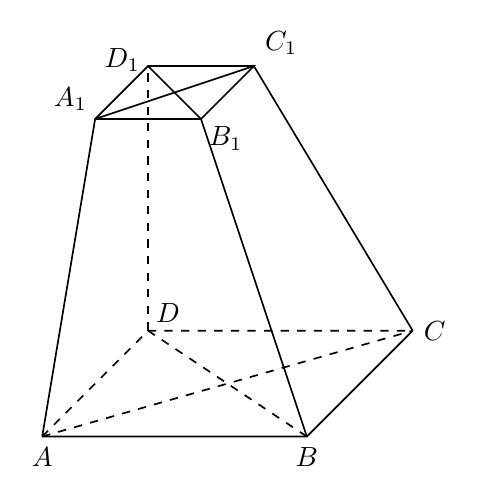
\begin{tikzpicture}[scale=1.12, semithick,
  every node/.style={inner sep=1.5pt}]
  \coordinate (A)  at (0,0);
  \coordinate (B)  at (3,0);
  \coordinate (C)  at (4.2,1.2);
  \coordinate (D)  at (1.2,1.2);
  \coordinate (A1) at (0.6,3.6);
  \coordinate (B1) at (1.8,3.6);
  \coordinate (C1) at (2.4,4.2);
  \coordinate (D1) at (1.2,4.2);
  % 被遮棱与底面辅助线
  \draw[dashed] (A) -- (D) -- (C);
  \draw[dashed] (D) -- (D1);
  \draw[dashed] (A) -- (C);
  \draw[dashed] (B) -- (D);
  % 可见棱
  \draw (A) -- (B) -- (C);
  \draw (C) -- (C1);
  \draw (A) -- (A1) -- (B1) -- (B);
  \draw (B1) -- (C1) -- (D1) -- (A1);
  % 上底面对角线
  \draw (A1) -- (C1);
  \draw (B1) -- (D1);
  % 顶点标注
  \node[anchor=north] at ([yshift=-2pt]A) {$A$};
  \node[anchor=north] at ([yshift=-2pt]B) {$B$};
  \node[anchor=west]  at ([xshift=2pt]C) {$C$};
  \node[anchor=south west] at ([xshift=1pt,yshift=1pt]D) {$D$};
  \node[anchor=south east] at ([xshift=-1pt,yshift=1pt]A1) {$A_1$};
  \node[anchor=north west] at ([xshift=1pt,yshift=-1pt]B1) {$B_1$};
  \node[anchor=south west] at ([xshift=2pt,yshift=2pt]C1) {$C_1$};
  \node[anchor=east] at ([xshift=-1pt,yshift=2pt]D1) {$D_1$};
\end{tikzpicture}
